\documentclass[unknownkeysallowed]{beamer}

\usepackage[utf8]{inputenc}
\usepackage[T1]{fontenc}
\usepackage[german]{babel}
\usepackage{graphicx} % Bilder
\usepackage{wrapfig} % Umflussbilder
\usepackage{multicol} % Multiple columns
\usepackage{minted} % Haskell source code
\usepackage{framed} % Frames around source code
\usepackage[framemethod=tikz]{mdframed} % Frames

\mdfdefinestyle{fancy}{
  roundcorner=5pt,
  linewidth=4pt,
  linecolor=red!80,
  backgroundcolor=red!20
}
\newmdenv[style=fancy]{important}

% Stuff for Beamer
\beamertemplatenavigationsymbolsempty
\usetheme{Madrid}

\begin{document}

%  \usebackgroundtemplate{\includegraphics[width=\paperwidth,height=\paperheight]{1.jpg}} 
  
%----------------------------------------------------------------------------------------  

  \begin{frame}
  \begin{center}
    \Huge\textbf{Fortgeschrittene funktionale Programmierung in Haskell}\\ \bigskip
    \LARGE Universität Bielefeld, Sommersemester 2015\\ \bigskip
    \large Jonas Betzendahl \& Stefan Dresselhaus
    \end{center}
  \end{frame}

%----------------------------------------------------------------------------------------  
  
\begin{frame}
\begin{center}
	\Large\textbf{\underline{Überblick für Heute:}}\\ \bigskip\bigskip\normalsize
	
	Organisatorisches\\\bigskip
	Tools \& Ressourcen\\\bigskip
	Thinking in Types\\\bigskip
	Functionally solving problems\\\bigskip
    \end{center}
\end{frame}

%----------------------------------------------------------------------------------------  
  
  \begin{frame}

    \begin{center}
    \Large\textbf{Organisatorisches}
    \end{center}
  \end{frame}

%----------------------------------------------------------------------------------------  
  
  \begin{frame}
    \begin{center}
    \Large\textbf{Organisatorisches: Veranstaltungen}\\ \bigskip \normalsize
    Es gibt Vorlesungen (Freitags, 14-16 Uhr in V2-205)\\
    und Übungen (Montags, 12-14 \& 18-20 Uhr in V2-221)\bigskip

	Vorlesungen aufgeteilt in \bigskip
	
	Teilnahme ist nicht verpflichtend, aber wahrscheinlich von Vorteil.  
    \end{center}
  \end{frame}
  
%----------------------------------------------------------------------------------------  
  
  \begin{frame}
    \begin{center}
    \Large\textbf{Organisatorisches (2): Input / Output}\\ \bigskip \normalsize
    
    Für das Modul gibt es 5 (echte) Leistungspunkte\\
    Als Leistung müsst ihr ein kleines Programmierprojekt abschließen.
    Details dazu in den Übungen.\bigskip
    
    Bürokratische Hürden $\Rightarrow$ Leistungspunkte nur für \emph{individuelle} Ergänzung.
    \end{center}
  \end{frame}
  
%----------------------------------------------------------------------------------------  
  
  \begin{frame}
    \begin{center}
    \Large\textbf{Organisatorisches (3): Personenkult}\\ \bigskip \normalsize

	Wir, das sind Jonas Betzendahl und Stefan Dresselhaus.\\
	Mailadressen: \texttt{\{jbetzend,sdressel\}@techfak\dots}\\ \bigskip
	Wir sind zwei Masterstudenten an der TechFak, die ihren Wunsch nach mehr und besserer Lehre zu funktionaler Programmierung und Haskell hier in Bielefeld jetzt selbst in die Hand nehmen. \bigskip    
    
    Formal verantwortlich ist Dr. Alexander Sczyrba (\texttt{asczyrba@techfak\dots}). Er ist eure Anlaufstelle für Fragen im Kontext der Fakultät und Beschwerden zu uns.
    \end{center}
  \end{frame}
  
%----------------------------------------------------------------------------------------  
  
  \begin{frame}
    \begin{center}
	\Large\textbf{Organisatorisches (4): Material von uns für euch}\\ \bigskip \normalsize
	Alle Übungsblätter, Foliensätze, Beispiele, Vorlagen und sonstige Unterlagen findet ihr entweder im ekVV oder auf der Website dieser Veranstaltung. Die URL ist:
	
	\bigskip\texttt{www.dieseurlmussnochersetztwerden.de}\bigskip
	
	Audio/Video-Mitschnitte findet ihr ebenfalls im Web und zwar auf folgender Seite:
	
	\bigskip\texttt{www.irgendwiesowaswieunirekorder.de}\bigskip
	
	Login: Login, Passwort: 123456
    \end{center}
  \end{frame}
  
%----------------------------------------------------------------------------------------  
  
  \begin{frame}

    \begin{center}
    \Large\textbf{Tools und Ressourcen}
    \end{center}
  \end{frame}
  
%----------------------------------------------------------------------------------------  
  
  \begin{frame}
    \begin{center}
    \Large\textbf{T \& R (1): Haskell / GHC}\\ \bigskip \normalsize
    
    Um auf euren eigenen Rechnern Haskell sinnvoll benutzen zu können benötigt ihr den \texttt{Glasgow Haskell Compiler} (GHC). \bigskip
    
    Der GHC und viele nützliche Dinge mehr sind alle im Rundum-Glücklich-Paket genannt \emph{Haskell Platform} enthalten. Die gibt es für Linux, Mac, BSD und Windows unter folgender URL:
    
    \bigskip\texttt{https://www.haskell.org/platform/}\smallskip
    
    \begin{important}
    \textbf{Wichtig:}\\ Der Interpreter \texttt{Hugs} wird von uns explizit \underline{nicht} unterstützt.
    \end{important}
    \end{center}
  \end{frame}
  
%----------------------------------------------------------------------------------------  
  
  \begin{frame}
    \begin{center}
    \Large\textbf{T \& R (2): GHCi}\\ \bigskip \normalsize
    
    Die mitgelieferte interaktive Umgebung des GHC heißt GHCi.\\\bigskip
    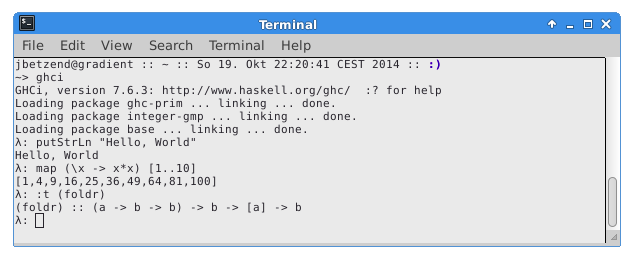
\includegraphics[scale=0.4]{ghci_example.png} 
    
    \bigskip Der GHCi stellt ein REPL (Read - Evaluate - Print - Loop) bereit, die beim Entwickeln \emph{sehr} nützlich sein kann (ähnlich zu \texttt{Hugs}). Mehr dazu in den Übungen.
    \end{center}
  \end{frame}
  
  %----------------------------------------------------------------------------------------  
  
  \begin{frame}
    \begin{center}
    \Large\textbf{T \& R (3): Hackage}\\ \bigskip \normalsize
    Dieser Tage gibt es eine Vielzahl an nützlichen und mächtigen Bibliotheken für Haskell. Zu Hause sind die meisten davon auf \emph{Hackage}: \\ \bigskip \texttt{https://hackage.haskell.org/} \\ \bigskip
    Auf Hackage findet ihr übersichtliche Zusammenfassungen der Bibliotheken, detaillierte Auflistungen der exportierten Funktionen und Datentypen und direkte Links zu den jeweiligen Implementationen (!).
    \end{center}
  \end{frame}
  
%----------------------------------------------------------------------------------------  
  
  \begin{frame}
    \begin{center}
    \Large\textbf{T \& R (4): cabal}\\ \bigskip \normalsize
    Ebenfalls in der \emph{Haskell Platform} enthalten ist \texttt{cabal}, Haskells eigenes Paket-Management-System. \texttt{cabal} erlaubt es euch, einfach via Terminal Bibliotheken von Hackage lokal (!) und im Zweifelsfall auch problemlos in einer Sandbox zu installieren. \texttt{cabal} ist außerdem ein Build-System, kann Test-Suites ausführen und und und. Aber auch dazu später mehr.\bigskip
    
    Das folgende Beispiel installiert \texttt{lens}, eine Bibliothek die uns im Lauf der Vorlesung noch begegnen wird:\bigskip
   
    \texttt{\$ cabal update \&\& cabal install lens}
    
    
    \end{center}
  \end{frame}
  
%----------------------------------------------------------------------------------------  
  
  \begin{frame}
    \begin{center}
    \Large\textbf{T \& R (5): LYAHFGG}\\ \bigskip \normalsize
    \begin{multicols}{2}
    
	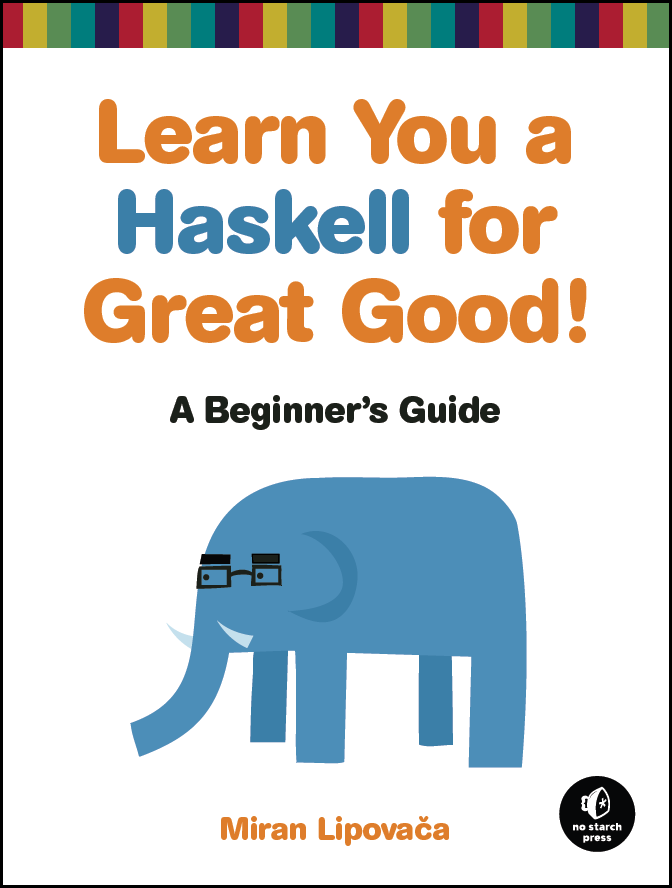
\includegraphics[scale=0.15]{lyah.png} 
	
	\columnbreak    
    Das Buch \glqq Learn You A Haskell\grqq\ ist die beste™ Ressource um die ersten Schritte in Haskell zu 
    lernen. Es ist verständlich und locker geschrieben und berühmt für gute Erklärungen.\bigskip
   
    Ihr findet es online frei und kostenlos verfügbar hier:
    
    \texttt{http://learnyouahaskell.com/}
    \end{multicols}
    \end{center}
  \end{frame}
  
%----------------------------------------------------------------------------------------  
  
  \begin{frame}
    \begin{center}
    \Large\textbf{T \& R (6): Hoogle}\\ \bigskip \normalsize
    \emph{Hoogle} ist eine Haskell-API-Suchmaschine, die es möglich macht, nach Funktionen zu suchen, ihren Typen angibt und zeigt, welche Imports nötig sind.\\ Ein besonders nützliches Feature ist, dass es auch möglich ist, nach Typsignaturen zu suchen und darauf passende Antworten zu erhalten.\\ \bigskip
    Die URL lautet: \texttt{http://www.haskell.org/hoogle/}
    \end{center}
  \end{frame}
  
%----------------------------------------------------------------------------------------  
  
  \begin{frame}

    \begin{center}
    \Large\textbf{Quer durch die Prelude \\ Thinking in Types}
    \end{center}
  \end{frame}
  
%----------------------------------------------------------------------------------------  
  
  \begin{frame}

    \begin{center}    
    Die Prelude ist Haskells Standardbibliothek und hat die wichtigsten Funktionen und Datentypen schon
    für euch zusammen gestellt. 
    \end{center}
  \end{frame}
  
%----------------------------------------------------------------------------------------  
  
  \begin{frame}[fragile]

    \begin{center}
    \Large\textbf{Die wichtigsten Typen...}\\
    
\begin{minted}[size=tiny]{haskell}
Bool          -- True, False
Int, Integer  -- 32bit und arbitrary precision
Float, Double -- Floating-point 
Char, String  -- Zeichen & Zeichenketten
              -- (String = [Char])
\end{minted}

\pause
\Large\textbf{... und Typkonstruktoren (polymorph)}\\

\begin{minted}[size=tiny]{haskell}             
[a]     -- Listen     
(a,b)   -- Tupel      
Maybe a -- Option type, "Just a" oder "Nothing"
\end{minted}

    \end{center}
\end{frame}

%----------------------------------------------------------------------------------------  
  
  \begin{frame}[fragile]

    \begin{center}
    \Large\textbf{QddP: Identity}\\\bigskip

\begin{minted}{haskell}
                  id :: a -> a
                  id x = x
\end{minted}

Typsignaturen, Polymorphismus, Pattern matching

    \end{center}
\end{frame}

%----------------------------------------------------------------------------------------  
  
  \begin{frame}[fragile]

    \begin{center}
    \Large\textbf{QddP: Konstanten}\\\bigskip

\begin{minted}{haskell}
                  const :: a -> b -> a
                  const x _ =  x
\end{minted}

Currying, wildcards

    \end{center}
\end{frame}

%----------------------------------------------------------------------------------------  
  
  \begin{frame}[fragile]

    \begin{center}
    \Large\textbf{QddP: Funktionsverkettung}\\\bigskip

\begin{minted}{haskell}
                  (.) :: (b -> c) -> (a -> b) -> a -> c
                  (.) f g = \x -> f (g x)
\end{minted}

Verkettung, Rechts nach Links lesen

    \end{center}
\end{frame}

%----------------------------------------------------------------------------------------  
  
  \begin{frame}[fragile]

    \begin{center}
    \Large\textbf{QddP: Booleans (1)}\\\bigskip

\begin{minted}{haskell}
                  data Bool = False | True
                  
                  not :: Bool -> Bool
                  not True = False
                  not _    = True
\end{minted}

    \end{center}
\end{frame}

%----------------------------------------------------------------------------------------  
  
  \begin{frame}[fragile]

    \begin{center}
    \Large\textbf{QddP: Booleans (2)}\\\bigskip

\begin{minted}{haskell}
                  (&&) :: Bool -> Bool -> Bool
                  (&&) True True = True
                  (&&) _    _    = False
                  
                  (||) :: Bool -> Bool -> Bool
                  (||) False False = False
                  (||) _     _     = True
\end{minted}

    \end{center}
\end{frame}

%----------------------------------------------------------------------------------------  
  
  \begin{frame}[fragile]

    \begin{center}
    \Large\textbf{QddP: Maybe (1)}\\\bigskip

\begin{minted}{haskell}
                  data Maybe a = Nothing
                               | Just a
\end{minted}

Tiefe etwa wie bei Bool

    \end{center}
\end{frame}

%----------------------------------------------------------------------------------------  
  
  \begin{frame}[fragile]

    \begin{center}
    \Large\textbf{QddP: Either (1)}\\\bigskip

\begin{minted}{haskell}
                  data Either a b = Left  a
                                  | Right b
\end{minted}

Tiefe etwa wie bei Bool

    \end{center}
\end{frame}

%----------------------------------------------------------------------------------------  
  
  \begin{frame}[fragile]

    \begin{center}
    \Large\textbf{QddP: Tuples}\\\bigskip

foobar

    \end{center}
\end{frame}

%----------------------------------------------------------------------------------------  
  
  \begin{frame}[fragile]

    \begin{center}
    \Large\textbf{QddP: Lists}\\\bigskip

foobar, Tiefe weiter als Maybe, Either, Bool

    \end{center}
\end{frame}

%----------------------------------------------------------------------------------------  
  
  \begin{frame}[fragile]

    \begin{center}
    \Large\textbf{QddP: basic IO}\\\bigskip

foobar, Verweis auf später

    \end{center}
\end{frame}


%----------------------------------------------------------------------------------------  
  
  \begin{frame}

    \begin{center}
    \Large\textbf{Solving problems by composition}
    \end{center}
  \end{frame}
  
%----------------------------------------------------------------------------------------  
  
  \begin{frame}

    \begin{center}
    \Large\textbf{Beispiel:}\bigskip
    
    \textbf{Aufgabe:} Sie bekommen einen Dateinamen übergeben. Lesen Sie die Datei Zeile für Zeile aus
    \end{center}
  \end{frame}
  
%----------------------------------------------------------------------------------------  
  
  \begin{frame}[fragile]

    \begin{center}
    \Large\textbf{Beispiel:}\\\bigskip

foobar: Lösung für Aufgabe in Haskell und C, mehr Beispiele

    \end{center}
\end{frame}
  
\end{document}